\documentclass{article}
\usepackage{graphicx} % Required for inserting images
\graphicspath{ {./images/} }
\usepackage{amsmath}
\usepackage{array}

\title{2. Gausa metode. Determinanti.}
\author{Gunārs Ābeltiņš}
\date{}

\begin{document}

\maketitle

\section*{Lekcijas konspekts}
Tika stāstīta par determinantiem. Kā tos aprēķināt. To īpašības.

\section*{1. Uzdevums}
\begin{equation*}
    \begin{cases}
        y + 3z + 8u = 4\\
        x + u = 2\\
        -2x + y - 2z = (-1)\\
        2y + z + 10u = 7
    \end{cases}
\end{equation*}

\begin{gather*}
    \left(
        \begin{tabular}{ c c c c|c }
            0 & 1 & 3 & 8 & 4\\
            1 & 0 & 0 & 1 & 2\\
            -2 & 1 & -2 & 0 & -1\\
            0 & 2 & 1 & 10 & 7
        \end{tabular}
    \right)
    \xrightarrow{r_1 \leftrightarrow r_2}
    \left(
        \begin{tabular}{ c c c c|c }
            1 & 0 & 0 & 1 & 2\\
            0 & 1 & 3 & 8 & 4\\
            -2 & 1 & -2 & 0 & -1\\
            0 & 2 & 1 & 10 & 7
        \end{tabular}
    \right)
    \xrightarrow{r_3 += 2r_1}
    \\
    \left(
        \begin{tabular}{ c c c c|c }
            1 & 0 & 0 & 1 & 2\\
            0 & 1 & 3 & 8 & 4\\
            0 & 1 & -2 & 2 & 1\\
            0 & 2 & 1 & 10 & 7
        \end{tabular}
    \right)
    \xrightarrow{
        \substack{
            r_3 -= 3r_2\\
            r_4 -= -2r_2
        }
    }
    \left(
        \begin{tabular}{ c c c c|c }
            1 & 0 & 0 & 1 & 2\\
            0 & 1 & 3 & 8 & 4\\
            0 & 0 & -5 & -6 & -1\\
            0 & 0 & -5 & -6 & -1
        \end{tabular}
    \right)
    \xrightarrow{x_3 /= (-5)}
    \\
    \left(
        \begin{tabular}{ c c c c|c }
            1 & 0 & 0 & 1 & 2\\
            0 & 1 & 3 & 8 & 4\\
            0 & 0 & 1 & 1.2 & 0.2\\
            0 & 0 & -5 & -6 & -1
        \end{tabular}
    \right)
    \xrightarrow{
        \substack{
            r_2 -= 3r_2\\
            r_4 += 5r_2
        }
    }
    \left(
        \begin{tabular}{ c c c c|c }
            1 & 0 & 0 & 1 & 2\\
            0 & 1 & 0 & 4.4 & 3.4\\
            0 & 0 & 1 & 1.2 & 0.2\\
            0 & 0 & 0 & 0 & 0
        \end{tabular}
    \right)
\end{gather*}

\begin{equation*}
    \begin{cases}
        x + u = 2\\
        y + 4.4u = 3.4\\
        z + 1.2u = 0.2
    \end{cases}
\end{equation*}

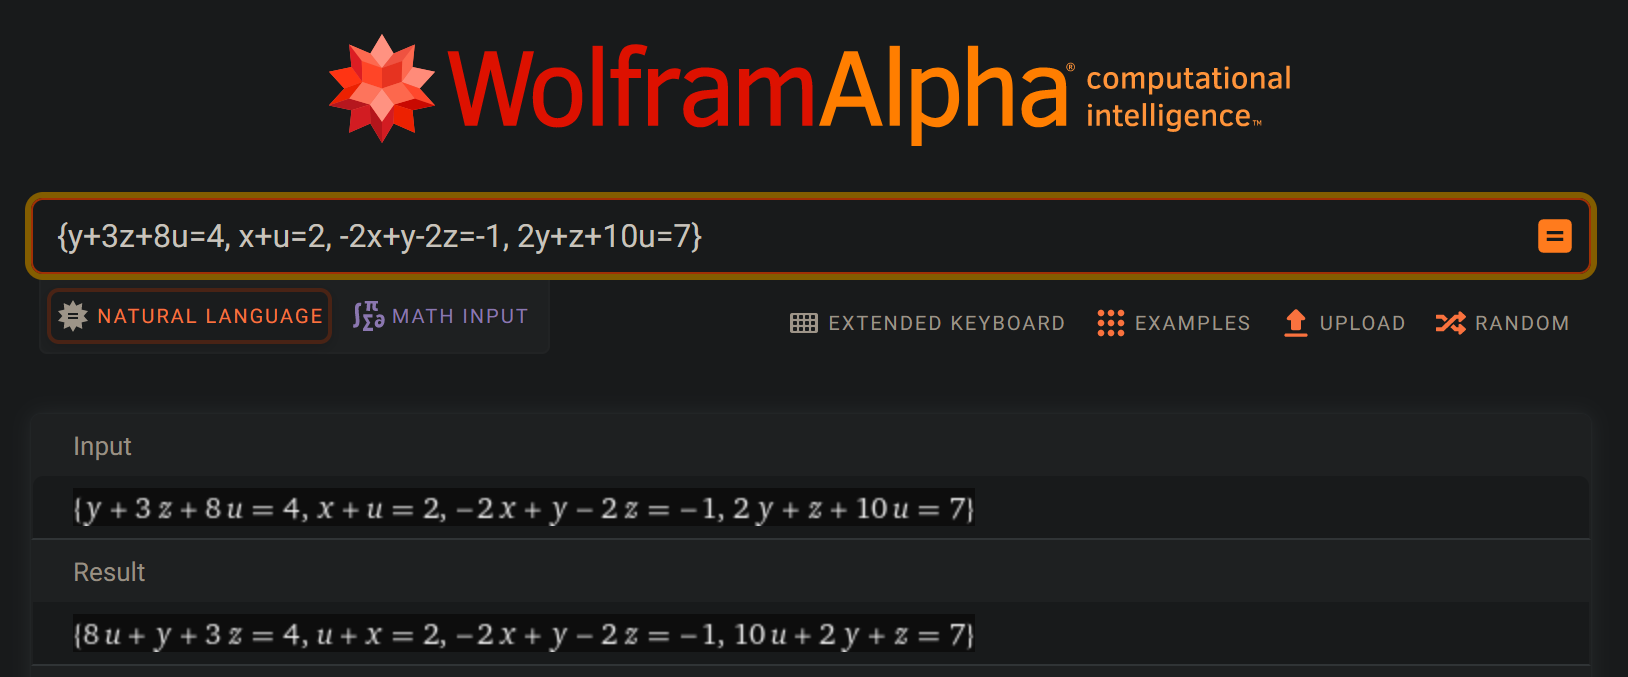
\includegraphics[width=\textwidth]{1}

\section*{2. Uzdevums}
\begin{equation*}
\det
\begin{pmatrix}
    8 & 5\\
    12 & 9
\end{pmatrix} 
 =
(8 \cdot 9) - (5 \cdot 12)
= 
72 - 60
=
12
\end{equation*}

\begin{equation*}
    \det
    \begin{pmatrix}
        -2 & 5\\
        -3 & -4
    \end{pmatrix} 
     =
    (-2 \cdot (-4)) - (5 \cdot (-3))
    = 
    8 - (-15)
    =
    23
\end{equation*}

\begin{equation*}
    \det
    \begin{pmatrix}
        a & 2a\\
        -2a & -3a
    \end{pmatrix} 
    = 
    (a \cdot (-3a)) - (2a \cdot (-2a))
    = 
    -3a^2 - (-4a^2)
    =
    a^2
\end{equation*}

\begin{equation*}
    \det
    \begin{pmatrix}
        a + b & b\\
        -b & a - b
    \end{pmatrix} 
    = 
    ((a + b) \cdot (a - b)) - (b \cdot (-b))
    = 
    (a^2 - b^2) - b^2
    =
    a^2
\end{equation*}

\section*{3. Uzdevums}
\begin{equation*}
    \begin{cases}
        13x -16y = 4\\
        -6x + 7y = 2
    \end{cases}
\end{equation*}

\begin{equation*}
    d 
    = 
    \begin{vmatrix}
        13 & -16\\
        -6 & 7
    \end{vmatrix}
    =
    91 - 96
    =
    -5
\end{equation*}

\begin{equation*}
    d_1
    = 
    \begin{vmatrix}
        4 & -16\\
        2 & 7
    \end{vmatrix}
    =
    28 - (-32)
    =
    60
\end{equation*}

\begin{equation*}
    d_1
    = 
    \begin{vmatrix}
        13 & 4\\
        -6 & 2
    \end{vmatrix}
    =
    26 - (-24)
    =
    50
\end{equation*}

\begin{equation*}
    x
    =
    \frac{d_1}{d}
    =
    \frac{60}{-5}
    =
    -12
\end{equation*}

\begin{equation*}
    y
    =
    \frac{d_2}{d}
    =
    \frac{50}{-5}
    =
    -10
\end{equation*}

\end{document}
